\documentclass[12pt,aspectratio=169]{beamer}

% 自訂字體的封包
\usepackage{fontspec}

% 導入圖形與表格的封包
\usepackage{graphicx}
\usepackage{booktabs}

% 提供進階數學環境與公式排版
\usepackage{mathtools, amsmath, amsfonts}

% 設定中文字體
\usepackage{xeCJK}
\setCJKmainfont{微軟正黑體}
\setmainfont{Times New Roman}
\XeTeXlinebreaklocale "zh"
\XeTeXlinebreakskip = 0pt plus 1pt

% 自訂字體顏色的封包
\usepackage{color}

% 自訂顏色
\definecolor{MyBlue}{RGB}{33, 73, 120}
\setbeamercolor{structure}{fg=MyBlue}
\setbeamercolor{title}{fg=MyBlue}

% (動畫)字會若隱若現的顯示
\beamersetuncovermixins{\opaqueness<1->{45}}{\opaqueness<1->{95}}

% 設定中文的標籤
\renewcommand{\figurename}{圖}
\renewcommand{\tablename}{表}

% 排版形式 
\mode<presentation>{
% 主題風格
\usetheme{Madrid}
% 主題顏色
\usecolortheme{Default}
% 主題字體
\usefonttheme{professionalfonts}
% itemize 及 item 的形狀
\setbeamertemplate{itemize items}[triangle]
\setbeamertemplate{itemize subitem}[circle]
\setbeamertemplate{itemize subsubitem}[square]

% 調整外框形式的字體大小
\setbeamerfont{headline}{size=\scriptsize}
\setbeamerfont{footline}{size=\scriptsize}
% 取消右下方的跳轉工具列
\setbeamertemplate{navigation symbols}{} 
% 自定義2：清除外框下緣但僅出頁碼
\setbeamertemplate{footline}[page number] 
% 設定頁面邊界
\setbeamersize{text margin left=0.8cm, text margin right=0.8cm}
\special{papersize=\the\paperwidth,\the\paperheight}
\providecommand{\tabularnewline}{\\}
}

\title{\Huge{黃丞暘}}
% \author{國立東華大學應用數學系統計碩士班}
% \institute{\large{應徵職位：瀚品數位科技有限公司|\,機率工程師}}
% \institute{\large{應徵職位：數轉院/綠色製程科技中心|\,AI數據分析師}}
% \institute{\large{應徵職位：新日興股份有限公司|【品保】客戶品質工程師 }}
% \institute{\large{\begin{tabular}{l}應徵職位：閎康科技股份有限公司\\\hspace{5em}專案工程師(Delayer 物化性樣品處理)\end{tabular}}}
% \institute{\large{應徵職位：怡利電子工業股份有限公司|\,QA工程師}}
% \institute{\large{應徵職位：覺揚股份有限公司|\,專案管理(PJM)}}
% \institute{\large{應徵職位： 欣銓科技股份有限公司|\,AI系統開發工程師}}
% \institute{\large{\begin{tabular}{l}應徵職位：台灣晶技股份有限公司\\\hspace{5em}【智能營運】AI應用分析工程師\end{tabular}}}
% \institute{\large{應徵職位： 欣興電子股份有限公司|\,PCB產品專案工程師}}
\institute{\large{應徵職位： 可成科技股份有限公司|\,品質保證(QA)工程師}}
% \institute{\large{應徵職位： 瀚宇博德股份有限公司|\,AI開發工程師}}

\date{June 10, 2026}

\begin{document}

% 封面
\begin{frame}
  \titlepage
\end{frame}

%---------------------------------
\begin{frame}{\textbf{自介}}
  \begin{columns}[T]
      % 左欄：文字
      \begin{column}{0.8\textwidth}
          \begin{description}
            \item[學歷：]國立東華大學應用數學系統計碩士班\\\vspace{0.5em}中山醫學大學心理學系
            \vspace{1em}
            \item[特質：]溝通表達、主動探索\&解決、領導力
            \vspace{1em}
            \item[正職：] 5 年以上教學經驗
            \vspace{1em}
            \item[兼職：]大學課程助教、計畫專案助理
            \vspace{1em}
            \item[語言：]多益 815（2025.12）
          \end{description}
      \end{column}

      % 右欄：頭像 + GitHub
      \begin{column}{0.25\textwidth}
          \centering
          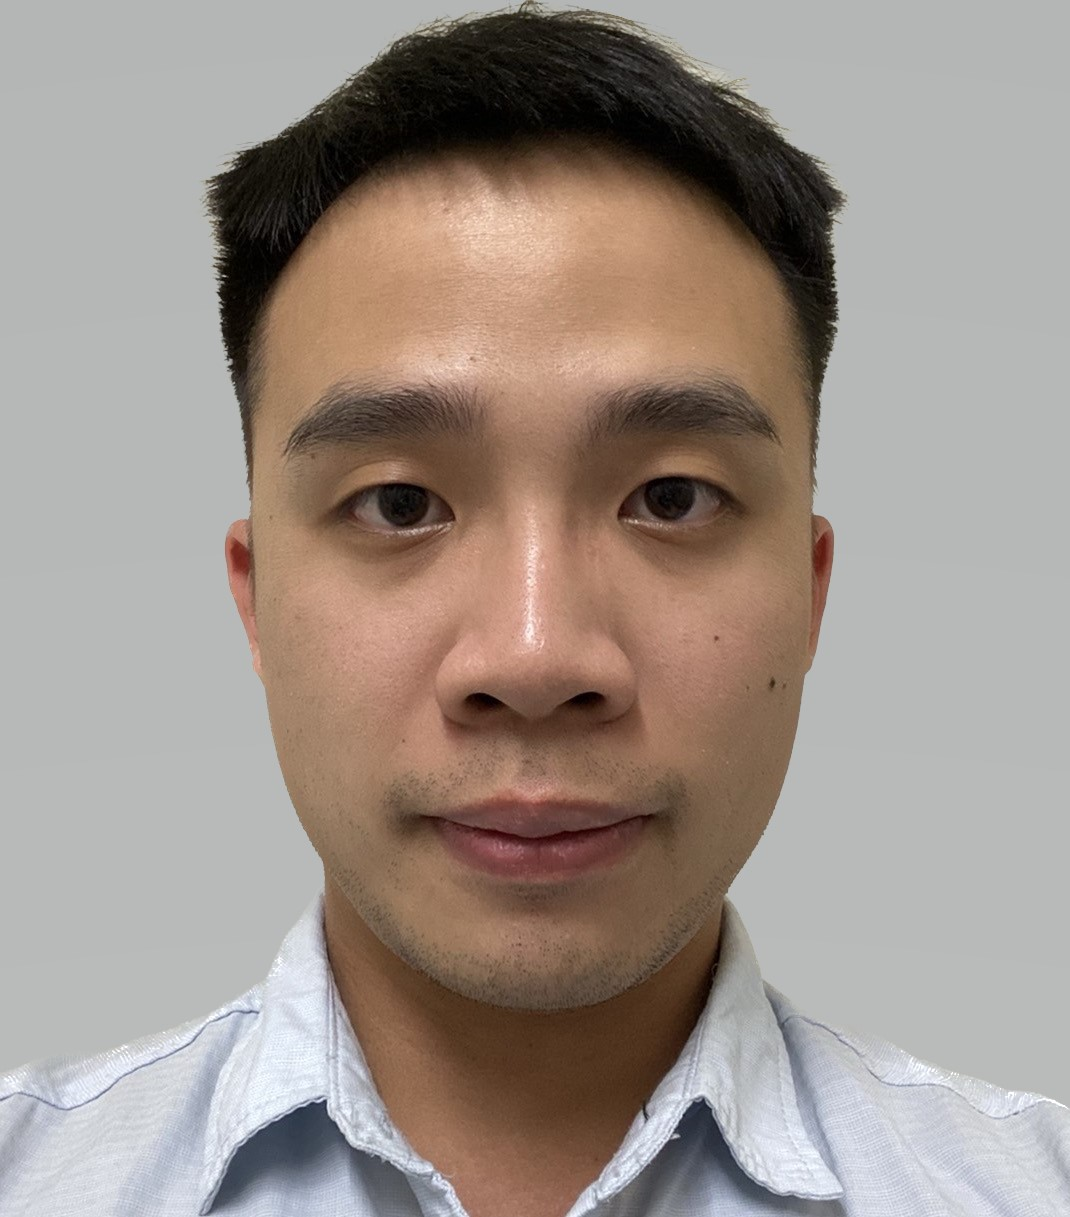
\includegraphics[width=0.6\linewidth]{大頭照_去背.jpg}

          \vspace{1em}

          {\small \href{https://github.com/JackHuang0125/WHAT_I_DID}{黃丞暘}}
      \end{column}
  \end{columns}
\end{frame}

%---------------------------------
\begin{frame}{\textbf{技能}}
  \begin{block}{統計分析}
    \begin{itemize}
      \item 假設檢定、統計推論、迴歸分析、ANOVA
    \end{itemize}
  \end{block}

  \begin{block}{Python}
    \begin{itemize}
      \item pandas、NumPy
      \item 視覺化：matplotlib
      \item 機器學習：scikit-learn、演算法、評估
      % \item 爬蟲：Beautiful Soup、Selenium
    \end{itemize}
  \end{block}

  % \begin{block}{SQL 資料庫基本查詢語法}
  %   \begin{itemize}
  %     \item WHERE、GROUP BY、JOIN ON、子查詢
  %   \end{itemize}
  % \end{block}

  \begin{block}{其他}
    \begin{itemize}
      \item SQL/R 基本語法、GitHub 版控、LaTex、文書處理
    \end{itemize}
  \end{block}
\end{frame}

%---------------------------------
\begin{frame}{\textbf{經驗與成果}}
  
  \begin{block}{\href{https://ppt.cc/fWdDdx}{統計諮詢課程}}
    \begin{itemize}
      \item 客戶需求釐清、問題定義、5分鐘 Pitch
      \item SPC 基礎、3$\sigma$ 理論
      \item 統計方法連結實務問題
    \end{itemize}
  \end{block}

  % \begin{block}{小型練習專案}
  %   \begin{itemize}
  %     % \item【記帳系統】使用 Python、FastAPI 與 PostgreSQL 建立後端 API
  %     \item【RAG問答系統】LangChain 串接 LLM，以 Streamlit 建置前端 UI
  %     \item【\href{https://socialworkerubing.streamlit.app/}{社工訪視紀錄系統}】使用 Streamlit、FastAPI 與 PostgreSQL 建置前後端，部署至 Cloud、Render、Neon
  %   \end{itemize}
  % \end{block}

  \begin{block}{\href{https://ppt.cc/f5zmzx}{教育大數據校內競賽（金牌）、2025資料科學漫步競賽}}
    \begin{itemize}
      \item 擔任隊長，使用 Python 進行資料分析、視覺化與統計檢定
    \end{itemize}
  \end{block}

  % \begin{block}{\href{https://ppt.cc/fLkv3x}{2025資料科學漫步競賽}}
  %   \begin{itemize}
  %     \item 擔任隊長，使用 Python 利用 MCA 降維、MANOVA 檢定、K-means 分群
  %   \end{itemize}
  % \end{block}
  
  \begin{block}{兼職－專案助理｜國⽴東華⼤學仿生環境工作坊}
    \begin{itemize}
       \item 使用 Google Site 管理團隊專案計畫相關⽂件與成果發表
       \item 撰寫國科會／縣政府計畫報告書各 1 份
       \item 規劃辦理 2024 科普環島列車花蓮站，當⽇活動⼈數達600
    \end{itemize}
  \end{block}

  % \begin{block}{兼職－課程助教｜國⽴東華⼤學應⽤數學系}
  %   \begin{itemize}
  %     \item 基礎機率、統計軟體、統計學
  %   \end{itemize}
  % \end{block}

\end{frame}

%---------------------------------
\begin{frame}{\textbf{論文研究　揭密黑箱模型－以半導體製程資料為例}}
  \begin{description}
    \item[問題：] 機器學習模型難以解釋資料的預測結果
    \vspace{1em}
    \item[資料：] 590 項特徵、缺失值、類別不平衡
    \vspace{1em}
    \item[方法：] 1. 建立迴歸線型模型解釋 XGBoost \\ 2. 優化計算效率
    \vspace{1em}
    \item[結果：] 1. 預測模型準確度達 9 成 、 刻劃模型 $R^2$ 達 7 成 \\ 2. 依模擬結果降低記憶體使用量達 9 成以及執行時間達 7成
    \vspace{1em}
    \item[價值：] 提供實務決策參考
  \end{description}
\end{frame}

%---------------------------------
\begin{frame}{\textbf{未來規劃}}
  \begin{block}{就職前準備}
    \begin{itemize}
      \item 學習貴公司 Domain Know-How
    \end{itemize}
  \end{block}
  \begin{block}{短期目標}
    \begin{itemize}
      \item 熟悉日常業務
      \item 提升個人能力
    \end{itemize}
  \end{block}
  \begin{block}{中期目標}
    \begin{itemize}
      \item 具有獨立執行專案的能力
      \item 把握外派機會
    \end{itemize}
  \end{block}
\end{frame}

%---------------------------------
\begin{frame}{\textbf{價值}}
  \begin{itemize}
    \item 具團隊溝通、客戶協調
    \vspace{1em}
    \item 具數學與統計背景
    \vspace{1em}
    \item 具程式語言基本使用概念
    \vspace{1em}
    \item 善用工具：ChatGPT、NotebookLM、Codex
  \end{itemize}
\end{frame}

%---------------------------------
\begin{frame}
  \vspace{3cm}
  \centering
  \Huge{\textbf{謝謝聆聽}}
  
  \vspace{3cm}
  \small\href{https://drive.google.com/file/d/1lE5E7IaBIESfK62EoWuBSgFOo_zypsXs/view?usp=sharing}{附件}
\end{frame}

\end{document}
